\documentclass[10pt,a4paper,titlepage]{article}
\usepackage[utf8]{inputenc}

\usepackage{amsmath}
\usepackage{amsfonts}
\usepackage{amssymb}
\usepackage{graphicx}
\usepackage{float} % force figure to render inline location
\usepackage{enumitem} % apt install texlive-latex-extra 
\usepackage{anyfontsize} % custom fontsizes
\usepackage{titlesec} % custom section spacings
\usepackage{multirow} % merge table rows
\usepackage{vhistory} % revision table package
\usepackage{pdfpages}
\usepackage{wrapfig}
\usepackage{lscape}
\usepackage{rotating}
\usepackage{epstopdf}
\usepackage{caption}
\usepackage{subcaption}
\usepackage{nameref} % allows use of named references

\setlist[itemize]{noitemsep} % No spaces in itemize lists
\setlist[enumerate]{noitemsep} % No spaces in itemize lists
\setlist[description]{noitemsep} % No spaces in itemize lists
\titlespacing*{\subsubsection}{0pt}{8pt}{2pt}
\titlespacing*{\paragraph}{0pt}{3pt}{5pt}

\newcommand{\cpright}{\textsuperscript{\tiny\copyright}}

\setlength\parindent{0pt}

\begin{document}
	
	\begin{titlepage}
		
		\title{
			\fontsize{50}{12}\selectfont{\textsc{Lunar Rover}}\\
			\vspace{20pt}
			\fontsize{20}{12}\selectfont{\textsc{Testing Summary}}\\
			\vspace{10pt}
			\large{Software Engineering \& Project} \\
			\vspace{20pt}
			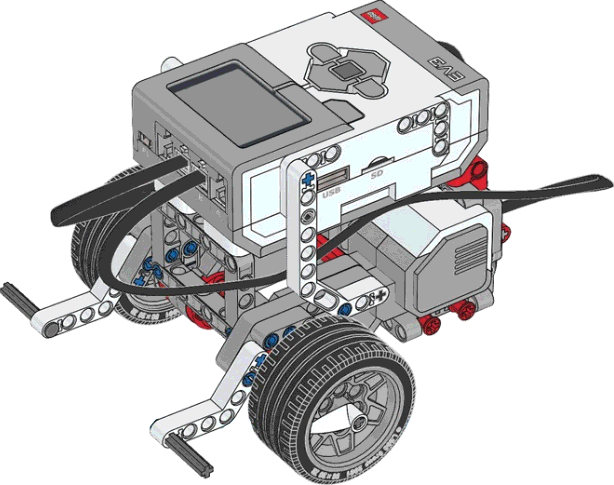
\includegraphics[width=200px]{title-page-ev3.png}					
		}
		\date{3/10/2017}
		\author{
			\bf{Team: PG-29} \\
			Kin Leong Lee \\
		}
		
	\end{titlepage}
		 
	\tableofcontents	
	\listoftables
		
	\section*{Revision History}	
	\label{revtable}	
	\begin{tabular}{|p{2.1cm}|p{2.5cm}|p{2cm}|p{4.1cm}|}		
		\hline 
		\textbf {Name} & \textbf{Date} & \textbf {Version} &\textbf {Summary of Changes} \\ \hline
		Issac Lee & 25-Oct-2017 & 0.11 & Fixed some symbols display issue and Revised the introduction and resource estimate sections\\ \hline
		\hline 
		\hline 		
	\end{tabular}

	\newpage	
	\section{Introduction}
		\subsection{Purpose}
		This Lunar Rover Test Report provides a summary of the results of test performed as outlined within this document. The software unit tests are running continuously thoroughly the development phases. The final acceptance test is running on 22-Oct-2017 and all type of tests will be running.
	
	\section{TEST SUMMARY}
\begin{itemize}
\item Project Name:  Lunar Rover
\item System Name: Michael Jackson
\item Version Number: 1.0
\end{itemize}
	\subsection{SOFTWARE UNIT TESTS}
	All unit tests are created by JUNIT and running on each development phase to ensure that the system can be running without any unexpected issue.
	\subsubsection{}
	\begin{itemize}
\item Test Owner:  Kin Leong Lee
\item Test Date: 22-Sep-2017
\item Test Description: To test the Event system can reference the difference unit object
\item Test Results: PASS – All objects are created successfully and referenced by event system
\item Additional Comments: This Test was running on each development phase. The final run is on 22-Oct-2017
	\end{itemize}

	\subsubsection{}
\begin{itemize}
\item Test Owner: Benjamin Charles Winding
\item Test Data: 27-Sep-2017
\item Test Description: To test whether service manager can be created
\item Test Results: PASS
\item Additional Comments: This Test was running on each development phase. The final run is on 22-Oct-2017
\end{itemize}

	\subsubsection{}	
\begin{itemize}
\item Test Owner: Huy Nguyen Phan
\item Test Data: 27-Sep-2017
\item Test Description: To test the software can successful enter manual mode and automatic mode
\item Test Results: PASS – Can return the appropriate value when the manual and automatic object are created.
\item Additional Comments: This Test was running on each development phase. The final run is on 22-Oct-2017
\end{itemize}

	\subsubsection{}
\begin{itemize}
\item Test Owner: Huy Nguyen Phan
\item Test Data: 10-Oct-2017
\item Test Description: To test the software can successful enter idle mode and way point mode
\item Test Results: PASS – Can return the appropriate value when the idle and way point object are created. Also, the position can also be returned correctly in way point mode.
\item Additional Comments: This Test was running on each development phase. The final run is on 22-Oct-2017
\end{itemize}

	\subsubsection{}
\begin{itemize}
\item Test Owner: Xiaoshan Chen
\item Test Data: 25-Sep-2017
\item Test Description: To test the colourtranslator class to ensure the color id can be returned correctly
\item Test Results: PASS – The color id can be matched to corresponding color name
\item Additional Comments: This Test was running on each development phase. The final run is on 22-Oct-2017
\end{itemize}

	\subsubsection{}
\begin{itemize}
\item Test Owner: Pavitterjeet Singh Sidhu
\item Test Data: 27-Sep-2017
\item Test Description: To test the sensorstate class to ensure the value \item from ultrasonic sensor can be returned correctly
\item Test Results: PASS – The value can be returned correctly
\item Additional Comments: This Test was running on each development phase. The final run is on 22-Oct-2017

\end{itemize}

	\subsubsection{}
\begin{itemize}
\item Test Owner: Sean Hennessy
\item Test Data: 20-Oct-2017
\item Test Description: To test the maptranslator object
\item Test Results: PASS – The system can read the XML file and output the XML file correctly  
\item Additional Comments: This Test was running on each development phase. The final run is on 22-Oct-2017

\end{itemize}

\subsection{INTEGRATION TEST IN SIMULATION ENVIRONMENT}
Software Manager - Huy Nguyen Phan established a program to simulate the robot can move correctly based on the reading from senesors.

	\subsubsection{}
\begin{itemize}
\item Test Owner:  Huy Nguyen Phan
\item Test Date: 22-Oct-201
\item Test Description: To detect radiation area 
\item Test Results: PASS
\item Additional Comments: The robot can detect radiation area and search the border on it
	
\end{itemize}

	\subsubsection{}
\begin{itemize}
\item Test Owner:  Xiaoshan Chen
\item Test Date: 22-Oct-201
\item Test Description: To detect Red color trail and follow this line
\item Test Results: PASS
\item Additional Comments:	
\end{itemize}

	\subsubsection{}
\begin{itemize}
\item Test Owner:  Kin Leong Lee
\item Test Date: 22-Oct-201
\item Test Description: To detect caters and avoid it
\item Test Results: PASS
\item Additional Comments:

\end{itemize}

	\subsubsection{}
\begin{itemize}
\item Test Owner:  Pavitterjeet Singh Sidhu
\item Test Date: 22-Oct-201
\item Test Description: To detect no-go zone in real time and avoid it
\item Test Results: PASS
\item Additional Comments:	
\end{itemize}

	\subsubsection{}
\begin{itemize}
\item Test Owner: Benjamin Charles Winding
\item Test Date: 22-Oct-201
\item Test Description: To detect no-go zone in real time and avoid it
\item Test Results: PASS
\item Additional Comments:

\end{itemize}

	\subsubsection{}
\begin{itemize}
\item Test Owner: Benjamin Charles Winding
\item Test Date: 22-Oct-201
\item Test Description: To detect the border and do not exceed the border
\item Test Results: PASS
\item Additional Comments:
\end{itemize}		
	
	\subsubsection{}
\begin{itemize}
\item Test Owner: Sean Hennessy
\item Test Data: 22-Oct-2017
\item Test Description: To detect a aplio and return to starting point
\item Test Results: PASS 
\item Additional Comments: 

\end{itemize}

	\subsubsection{}
\begin{itemize}
\item Test Owner:  Huy Nguyen Phan
\item Test Date: 22-Oct-201
\item Test Description: To detect obstacle and avoid it 
\item Test Results: PASS
\item Additional Comments	
\end{itemize}

\subsection{INTEGRATION TEST IN USER ENVIRONMENT}
	\subsubsection{}
\begin{itemize}
	\item Test Owner:  Huy Nguyen Phan
	\item Test Date: 22-Oct-201
	\item Test Description: To detect radiation area 
	\item Test Results: FAIL
	\item Additional Comments: The color sensor is not sensitive enough to distinguish green and blue
	
\end{itemize}

\subsubsection{}
\begin{itemize}
	\item Test Owner:  Xiaoshan Chen
	\item Test Date: 22-Oct-201
	\item Test Description: To detect Red color trail and follow this line
	\item Test Results: PASS
	\item Additional Comments:	
\end{itemize}

\subsubsection{}
\begin{itemize}
	\item Test Owner:  Kin Leong Lee
	\item Test Date: 22-Oct-201
	\item Test Description: To detect caters and avoid it
	\item Test Results: PASS
	\item Additional Comments:
	
\end{itemize}

\subsubsection{}
\begin{itemize}
	\item Test Owner:  Pavitterjeet Singh Sidhu
	\item Test Date: 22-Oct-201
	\item Test Description: To detect no-go zone in real time and avoid it
	\item Test Results: PASS
	\item Additional Comments:	
\end{itemize}

\subsubsection{}
\begin{itemize}
	\item Test Owner: Benjamin Charles Winding
	\item Test Date: 22-Oct-201
	\item Test Description: To detect no-go zone in real time and avoid it
	\item Test Results: PASS
	\item Additional Comments:
	
\end{itemize}

\subsubsection{}
\begin{itemize}
	\item Test Owner: Benjamin Charles Winding
	\item Test Date: 22-Oct-201
	\item Test Description: To detect the border and do not exceed the border
	\item Test Results: FAIL
	\item Additional Comments:The color sensor is not sensitive enough to distinguish green and blue
\end{itemize}		

\subsubsection{}
\begin{itemize}
	\item Test Owner: Sean Hennessy
	\item Test Data: 22-Oct-2017
	\item Test Description: To detect a aplio and return to starting point
	\item Test Results: PASS 
	\item Additional Comments: 
	
\end{itemize}

\subsubsection{}
\begin{itemize}
	\item Test Owner: Benjamin Charles Winding
	\item Test Date: 22-Oct-201
	\item Test Description: To detect obstacle and avoid it 
	\item Test Results: PASS
	\item Additional Comments	
\end{itemize}
	
\subsection{TEST RESULTS}
The testing result is acceptable. However, regarding integration test cases running in user environment, the testing result is not satisfactory since the color sensor is not sensitive enough to detect the correct color

\subsection{SUGGESTED ACTIONS}



\end{document}